\begin{figure}
	\centering
	\includegraphics[width=0.85\linewidth]{FIGS/fig-simplified-arch.png}
	\caption{\small Edge Offload Pipeline}
	\label{fig:e2epipeline}
\end{figure}

\begin{figure}
	\definecolor{observe-color}{RGB}{175,208,149}
	\definecolor{orient-color}{RGB}{255, 255, 166}
	\definecolor{decide-color}{RGB}{255,170,149}
	\definecolor{act-color}{RGB}{224,194,205}
	\centering
	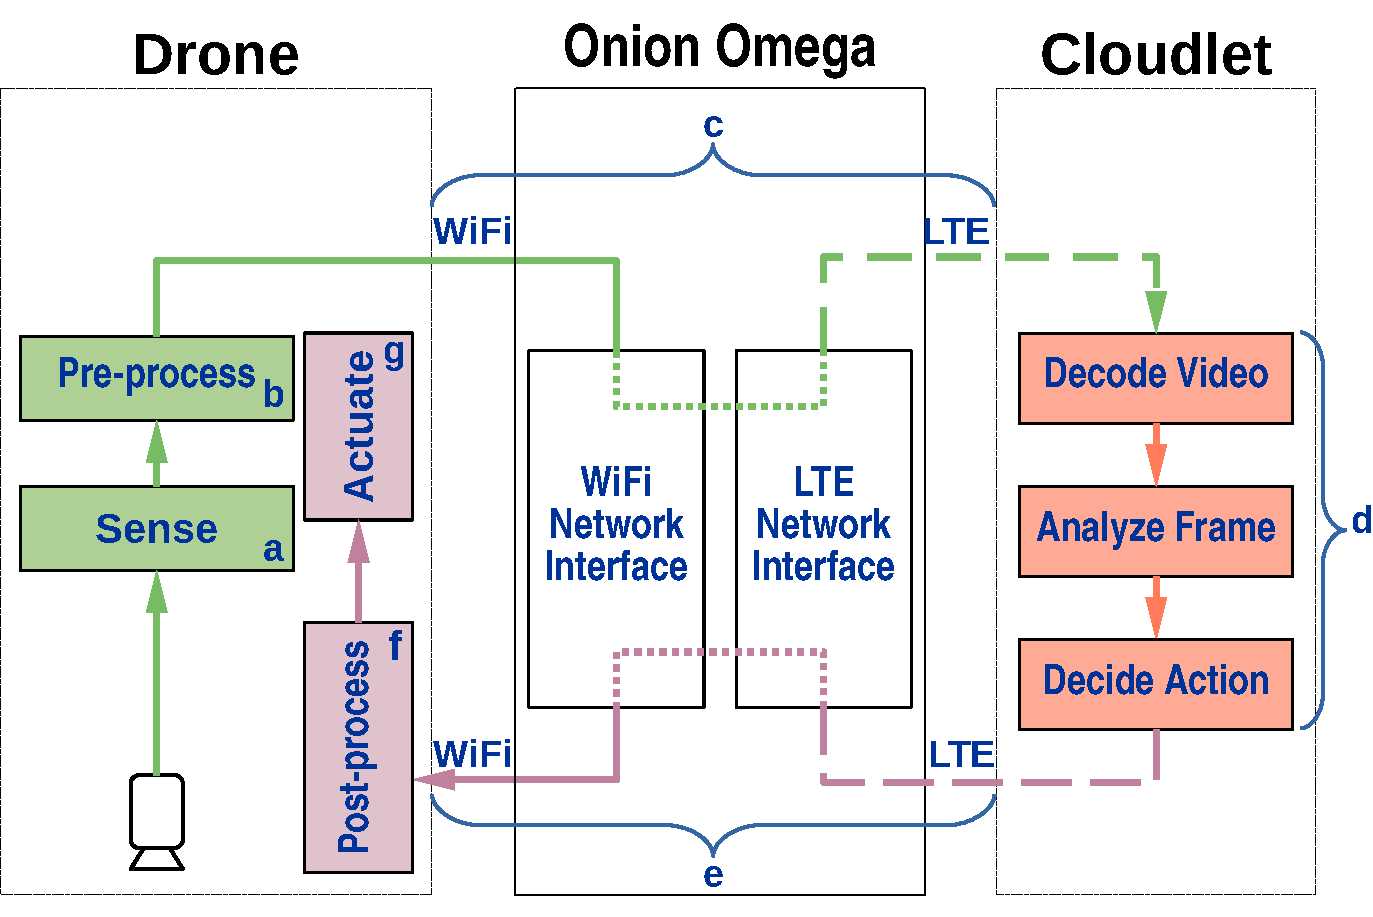
\includegraphics[width=0.9\linewidth]{FIGS/fig-ooda-loop.pdf}
	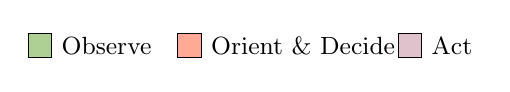
\begin{tikzpicture}
	    \draw[fill=observe-color] (1.0,0) rectangle (1.3,0.3);
	    \node[right] at (1.3,0.15) {\small Observe};
	
	    \draw[fill=decide-color] (2.9,0) rectangle (3.2,0.3);
	    \node[right] at (3.2,0.15) {\small Orient \& Decide};
	
	    \draw[fill=act-color] (5.7,0) rectangle (6.0,0.3);
	    \node[right] at (6.0,0.15) {\small Act};
	\end{tikzpicture}
	\caption{\small Detailed View of Our OODA Loop}
	\label{fig:ooda-loop}
	\vspace{0.2in}
	\centering
	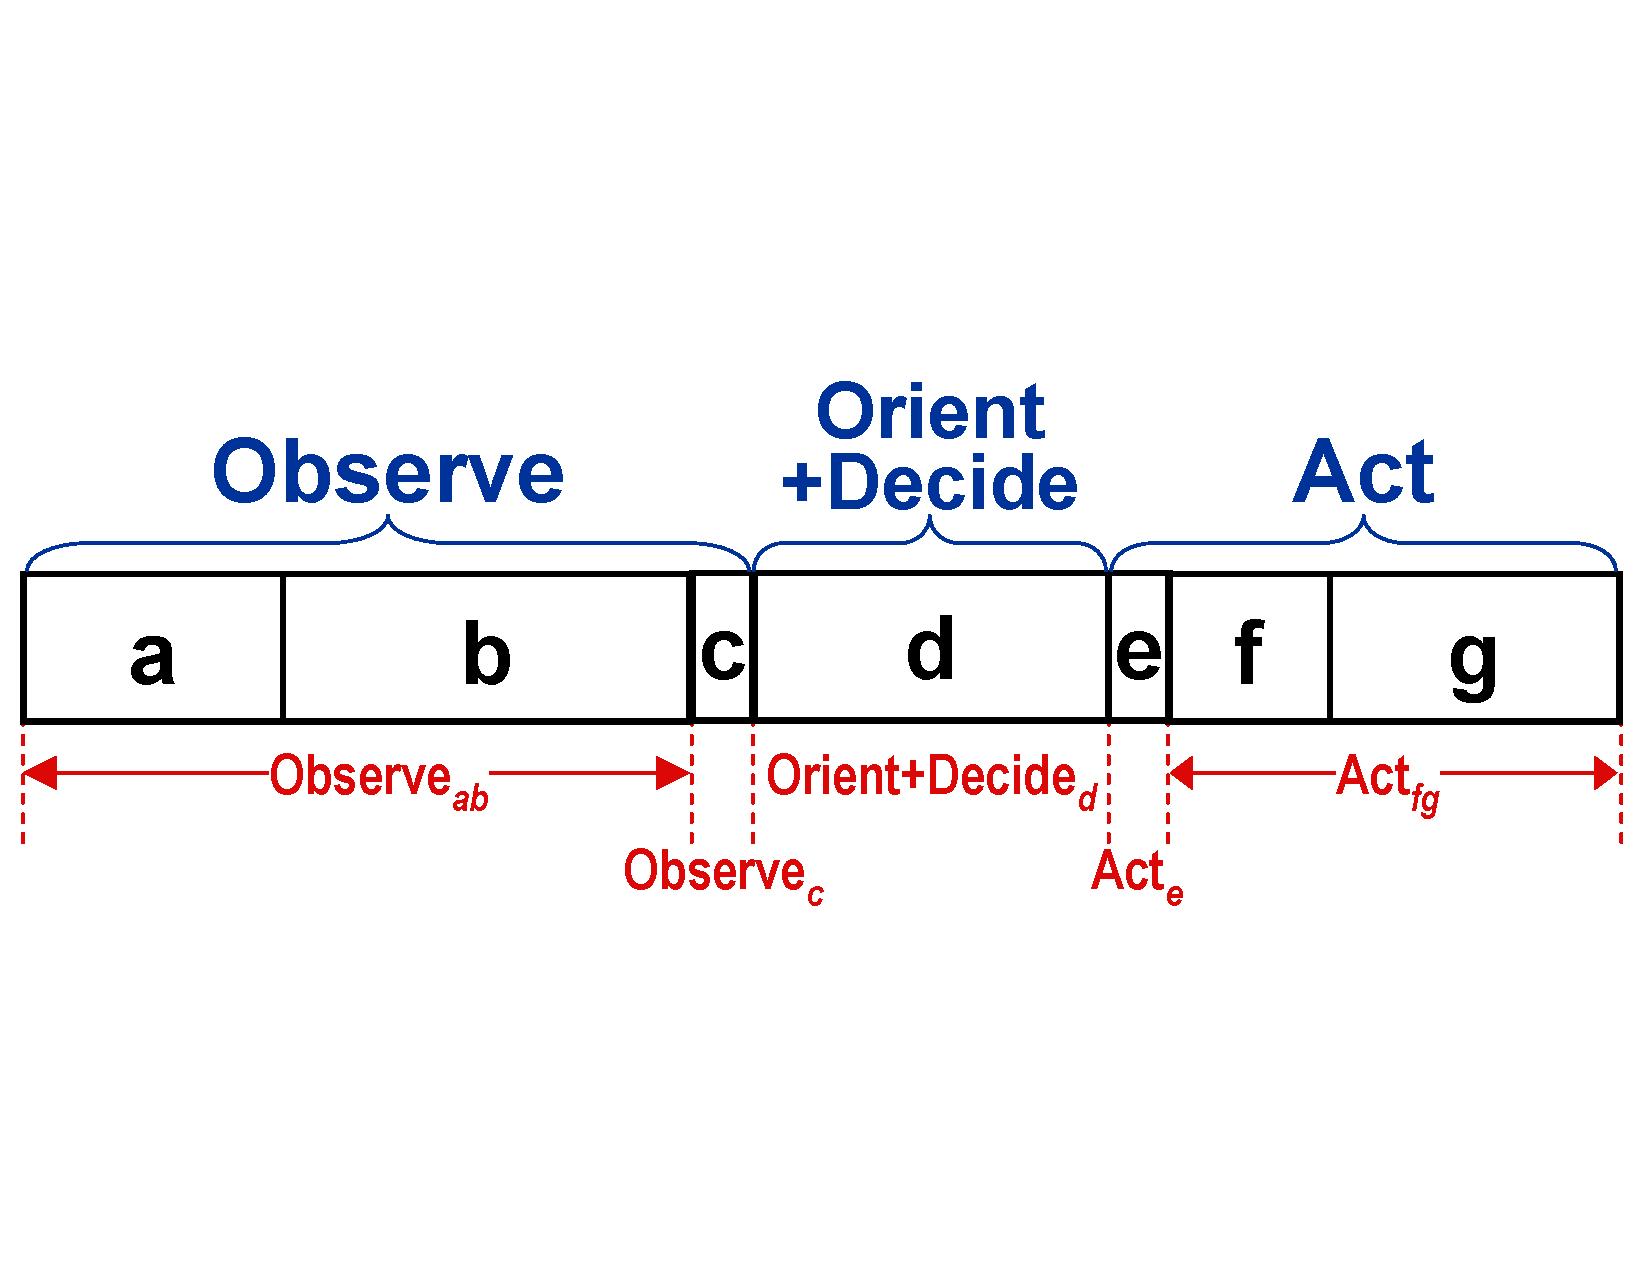
\includegraphics[width=0.9\linewidth]{FIGS/fig-ooda-nomenclature.pdf}
	\begin{captext}
		\centering Only items in \textcolor{red}{red} above can be measured.
		\flushleft
		\begin{tabular}{lll}
			\phantom{00} & a = on-drone sensing & e = transmission to drone\\
			\phantom{00} & b = on-drone pre-processing & f = on-drone post-processing\\
			\phantom{00} & c = transmission to cloudlet & g = drone actuation\\
			\phantom{00} & d = processing on cloudlet\\
		\end{tabular}
	\end{captext}
	\vspace{-0.1in}
	\caption{\small Measurable Components of Our OODA Loop}
	\label{fig:nomenclature}

\end{figure}

\section{Profiling \& Optimizing the \ooda~  Loop}
\label{sec:e2e-latency}

We replicate the setup~(Figure~\ref{fig:e2epipeline}) described by
Bala et al~\cite{Bala2023} using a slightly larger and heavier
variant~(550~g vs. 360~g) of the Parrot ANAFI drone. This variant is
approved on the BlueUAS list~\cite{BlueUAS2024} for US government
applications. As payload, we use the 53~g Onion Omega 2
LTE~\cite{Omega2023} single board computer which was briefly described
in that paper. The Onion Omega receives the sensor stream from the
drone over WiFi and forwards it to the cloudlet over 4G LTE.  The resulting
computation for Orient and Decide (e.g. DNN model
inference) causes a control message to be sent back via 4G LTE
to the Onion Omega, and thence over WiFi to the drone.

The drone to cloudlet pipeline is used for both data plane
and control plane operations.  Its intrinsic end-to-end performance
defines the experimental baseline.  To explore pipeline degradation,
we add network latency using FireQoS ~\cite{FireQoS} and drop frames
to throttle bandwidth.

\subsection{Mapping the OODA Loop}
\label{sec:mapping}

Figure~\ref{fig:ooda-loop} maps our end-to-end pipeline to \ooda~loop
components.  Components (a), (b) and (c) together map to the
``Observe'' phase; component (d) maps to its ``Orient'' and
``Decide'' phases; and, components (e), (f) and (g) together map to
the ``Act'' phase.  Due to closed-source restrictions of our COTS
pipeline, some \ooda~loop components have to be aggregated for
purposes of measurement, as shown by Figure~\ref{fig:nomenclature}.
Total end-to-end latency is given by the sum of these components;
total throughput is that of its bottleneck.

The earliest point in the pipeline where software instrumentation can
be inserted is between the Wi-Fi and LTE interfaces on the Onion
Omega.  The Wi-Fi part of this pipeline is thus attributed to
Observe$_{ab}$ rather than to Observe$_{c}$.  Similarly, on the return
path, the Wi-Fi part is attributed to Act$_{fg}$ rather than to
Act$_{e}$. Only LTE transmission is attributed to Observe$_{c}$ and
Act$_{e}$.  The resulting error is likely to be very small since Wi-Fi
is much more performant than LTE.  We present our detailed
measurements in \S\ref{sec:d2c-drone} to \S\ref{sec:c2d-drone}.


\subsection{Observe$_{ab}$}
\label{sec:d2c-drone}

Our drone is a commercial product that uses black box hardware and
software to seamlessly integrate (a) and (b).  Its camera creates a
stream of raw video frames.  On-board processing transforms these raw
frames into a sequence of UDP packets that slice-encode a 720p H.264
RTSP video stream at 30~fps~\cite{Schulzrinne2016}.  Neither the
resolution nor frame rate of this video stream are configurable.  The
slice encoding aims to reduce the visual impact of UDP packet loss.
The black box nature of this transformation makes attribution of
latency costs difficult.  It is not possible to insert instrumentation
to separate (a) and (b); they merge into an indivisible component.

\begin{figure}
\centering

\begin{minipage}[b]{.49\linewidth}
\centering
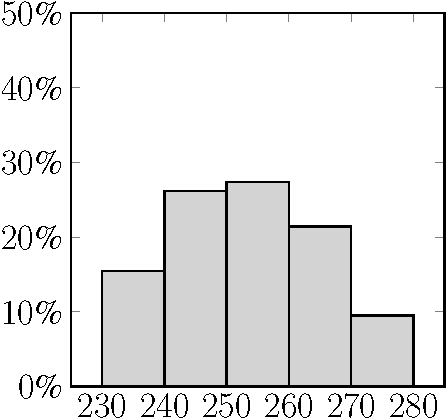
\includegraphics[width=0.97\linewidth]{histo-observeab-latency.pdf}
\begin{captext}
\centering
Mean: 253 $\pm 12$~ms\; p99: 277~ms\\
\end{captext}
\vspace{-0.05in}
{\small (a) Latency (ms)}
\end{minipage}
\begin{minipage}[b]{.49\linewidth}
\centering
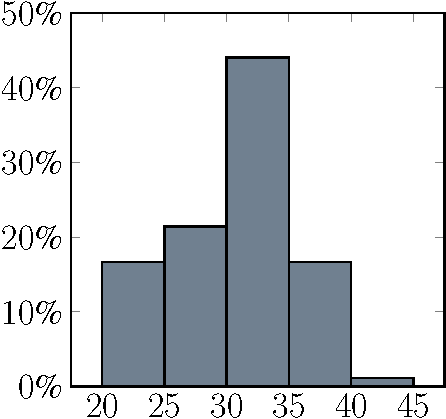
\includegraphics[width=0.97\linewidth]{histo-observeab-throughput.pdf}
\begin{captext}
\centering
Mean: 31~$\pm$5~fps\; p1: 22~fps\\
\end{captext}
\vspace{-0.05in}
{\small (b) Instant. Throughput (fps)}
\end{minipage}
\caption{\small Observe$_{ab}$ Measurements}
\label{fig:d2c-drone-histo}
\vspace{-0.1in}
\end{figure}

Figure~\ref{fig:d2c-drone-histo} presents our measurements.  The
latency distribution has a mean of 253~ms, with a standard deviation
of 12~ms and a p99 of 277~ms.  Instantaneous throughput has a mean of
31~fps, with a standard deviation of 5~fps and a p1 of 22~fps.  Due to
streaming, throughput can be higher than the reciprocal of latency.
The short WiFi Observe$_{ab}$ segment is partly responsible for this observed variation.

\subsection{Observe$_c$}
\label{sec:netdownlink}

As Figure~\ref{fig:e2epipeline} illustrates, the wireless network path
from drone to cloudlet consists of a very short Wi-Fi segment, transit
through the Onion router carried as payload, and then a longer 4G~LTE
segment to the cloudlet.  Figure~\ref{fig:d2c-net} presents the
latency and throughput distributions of Observe$_c$.  Its latency has
a mean of 39~ms, with a standard deviation of 8~ms and a p99 of 60~ms.
Instantaneous throughput has a mean of 16.3~Mbps, with a standard
deviation of 1~Mbps and a p1 of 14.4~Mbps.  Since 720p video at 30~fps
only demands an average bit rate of about 6.5~Mbps~\cite{Adobe2024},
Observe$_c$ is definitely not the bottleneck.


\begin{figure}
\vspace{0.1in}
\centering
\begin{minipage}[b]{.49\linewidth}
\centering
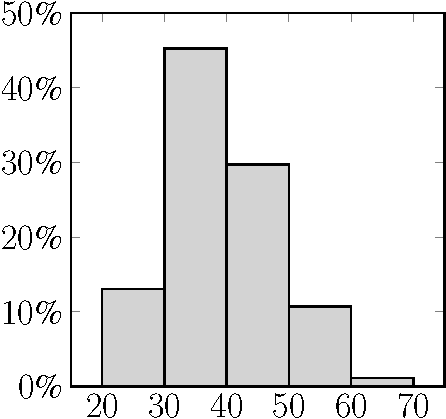
\includegraphics[width=0.97\linewidth]{histo-observec-latency.pdf}\\
\begin{captext}
\centering
Mean: 39~$\pm$8~ms\;p99: 60~ms\\
\end{captext}
\vspace{-0.05in}
{\small (a) Latency (ms)}
\end{minipage}
\begin{minipage}[b]{0.49\linewidth}
\centering
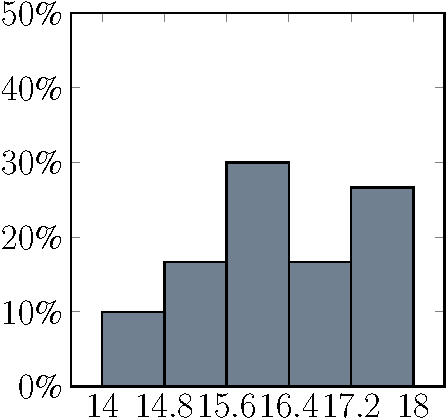
\includegraphics[width=0.97\linewidth]{histo-observec-throughput.pdf}\\
\begin{captext}
\centering
Mean: 16.3$\pm$1~Mbps p1: 14.4Mbps
\end{captext}
{\small (b) Throughput (Mbps)}
\end{minipage}
\vspace{-0.1in}
\caption{\small Observe$_c$ Measurements}
\label{fig:d2c-net}
\end{figure}

\subsection{Orient+Decide$_d$}
\label{sec:cloudlet}

Processing on the cloudlet involves three stages:
\begin{smitemize}

\item{Stage-1: Decoding the UDP packet stream to produce individual
    frames from H.264 video.}

\item{Stage-2: Application-specific processing of each frame to
    interpret its contents.  For example, this could involve DNN
    inferencing with a pre-trained model to detect objects of
    interest currently visible to the drone.}

\item{Stage-3: Application-specific logic to determine salient changes
    revealed by Stage-2.  This early part of Stage-3, together with
    Stage-1 and Stage-2, constitute the ``Orient'' part of the
    \ooda~loop.  The rest of Stage-3 is the ``Decide'' part. Drone
    actuation (if any) is determined, and the command to perform this
    actuation is generated.  For example, Stage-2 may show that an
    object being tracked has moved and the gimbal has to be adjusted
    to re-center the object in the camera's field of view~(FOV).}
\end{smitemize}
Stage-2 can be viewed as perception and Stage-3 as cognition.  The
latency and throughput of Stage-1 constrain the performance of
Orient+Decide$_d$ since decoding has to be performed even if Stage-2
and Stage-3 take a negligible amount of time.


\begin{figure}
\centering
\begin{minipage}[b]{0.49\linewidth}
\centering
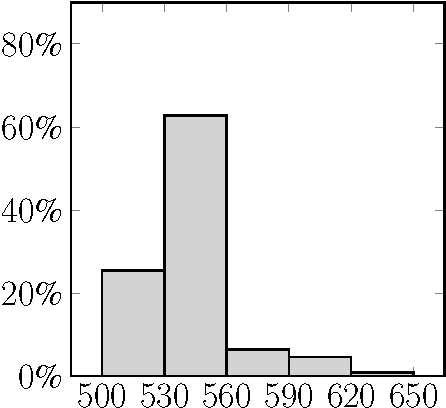
\includegraphics[width=0.97\linewidth]{histo-stage1-latency.pdf}\\
\begin{captext}
\centering
Mean: 541~$\pm$22~ms\hspace{0.1in}p99: 620~ms\\
\end{captext}
\vspace{-0.05in}
{\small (a) Latency (ms)}
\end{minipage}
\begin{minipage}[b]{0.49\linewidth}
\centering
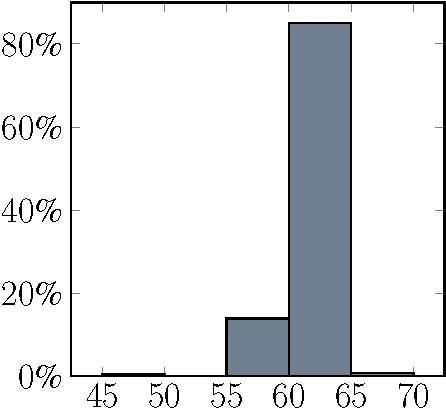
\includegraphics[width=0.97\linewidth]{histo-stage1-throughput.pdf}\\
\begin{captext}
\centering
Mean: 62~$\pm$1.5~fps\hspace{0.1in}p1: 59~fps\\
\end{captext}
\vspace{-0.05in}
{\small (b) Instant. Throughput (fps)}
\end{minipage}
\vspace{-0.15in}
\caption{\small Original FFmpeg-based Stage-1 Performance}
\label{fig:stage1-histo}
\vspace{-0.1in}
\end{figure}


Figure~\ref{fig:stage1-histo} presents our measurements of Stage-1. We
were surprised by the magnitude of the latency, with a mean of 541~ms.
Our cloudlet has two Intel Xeon processors with a total of 36 cores,
128GB of RAM and an NVIDIA GeForce GTX 1080 Ti GPU. This should be
ample for efficient software decoding of an H.264 video stream, as
confirmed by the mean throughput of 62~fps shown in
Figure~\ref{fig:stage1-histo}(b).  The high latency observed has no
obvious explanation, but it has a large negative impact on the
\ooda~pipeline.  As detailed elsewhere~\cite{Chanana2024}, we
determined that the culprit was negative latency scaleout of FFmpeg
when performing single stream
decoding~(Figure~\ref{fig:ffmpeg-threads-box-plot2}).

By switching to  different decoding software~\cite{PDrAW2024}, we
were able to reduce the latency from a mean of 541~ms in
\Cref{fig:stage1-histo}(a) to a mean of 32~ms in
\Cref{fig:pdraw-histo}(a).  This has been achieved with a mean
throughput of 37~fps~(\Cref{fig:pdraw-histo}(b)), which is well above
the demand of 31~fps from Observe$_{ab}$.  Assuming negligible
processing in Stage-2 and Stage-3, Figure~\ref{fig:pdraw-histo} shows
the best-case latency and throughput of Orient+Decide$_d$.

\begin{figure}
\centering
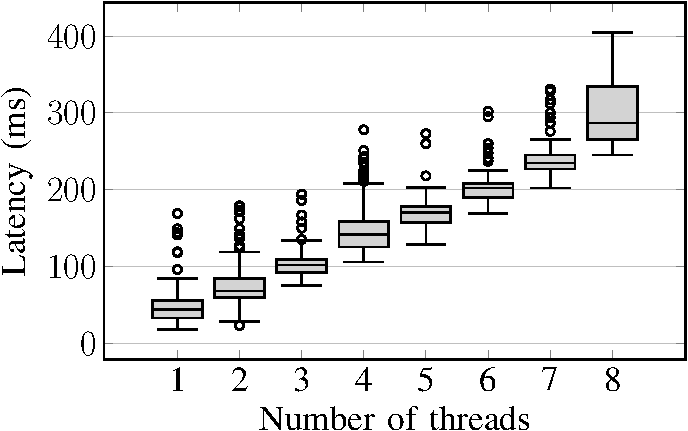
\includegraphics[width=0.75\linewidth]{histo-multi-threaded-ffmpeg.pdf}
\begin{captext}
  Each box extends from the first quartile ($Q_1$) to the third
  quartile ($Q_3$), with a line at the median. Whiskers extend from
  the box to the farthest data point lying within 1.5x the
  inter-quartile range ($IQR = Q_3-Q_1$) from the box. Circles
  represent outliers.
\end{captext}
\vspace{-0.1in}
\caption{\small Negative Scale-out of FFmpeg Latency}
\label{fig:ffmpeg-threads-box-plot2}
\end{figure}


\begin{figure}
\centering
\begin{minipage}[b]{0.49\linewidth}
\centering
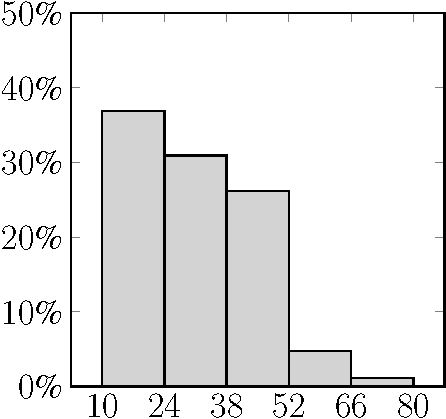
\includegraphics[width=0.97\linewidth]{histo-pdraw-latency.pdf}\\
\begin{captext}
\centering
Mean: 32~$\pm$13~ms\hspace{0.1in}p99: 59~ms\\
\end{captext}
{\small (a) Latency (ms)}
\end{minipage}
\begin{minipage}[b]{0.49\linewidth}
\centering
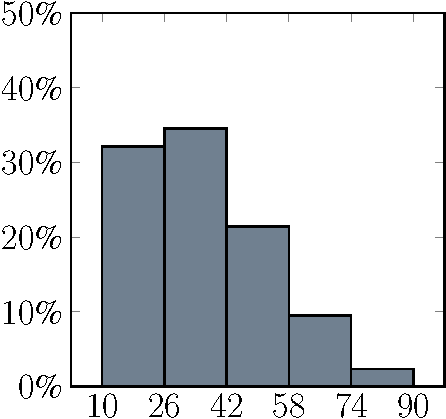
\includegraphics[width=0.97\linewidth]{histo-pdraw-throughput.pdf}\\
\begin{captext}
\centering
Mean: 37~$\pm$16~fps\hspace{0.1in}p1: 17~fps\\
\end{captext}
{\small (b) Instant. Throughput (fps)}
\end{minipage}
\vspace{-0.1in}
\caption{\small Improved Performance With FFmpeg Alternative}
\label{fig:pdraw-histo}
\vspace{-0.1in}
\end{figure}

\begin{figure}
\centering
\begin{minipage}[b]{0.49\linewidth}
\centering
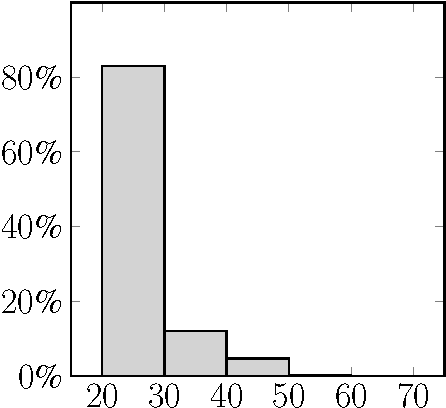
\includegraphics[width=0.97\linewidth]{histo-acte-latency.pdf}\\
\begin{captext}
\centering
Mean: 30~$\pm$4~ms\hspace{0.1in}p99: 49~ms\\
\end{captext}
{\small (a) Latency (ms)}
\end{minipage}
\begin{minipage}[b]{0.49\linewidth}
\centering
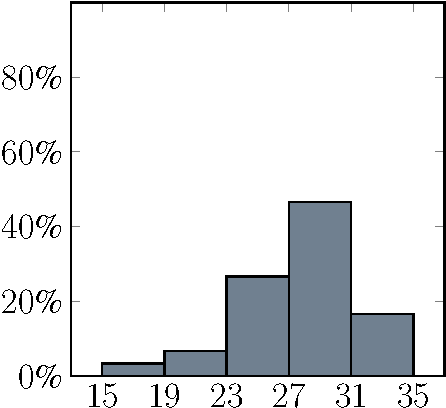
\includegraphics[width=0.97\linewidth]{histo-acte-throughput.pdf}\\
\begin{captext}
\centering
Mean: 28$\pm$3.7~Mbps p1: 19~Mbps\\
\end{captext}
{\small (b) Throughput (Mbps)}
\end{minipage}
\vspace{-0.15in}
\caption{\small Act${_e}$ Measurements}
\label{fig:c2d-net}
\end{figure}


\subsection{Act$_e$}
\label{sec:netuplink}

Figure~\ref{fig:c2d-net} presents our measurements of the wireless
network path from cloudlet to drone.  The latency has a mean of 30~ms,
with a standard deviation of 4~ms and a p99 of 49~ms.  The throughput
has a mean of 28~Mbps, with a standard deviation of 3.7~Mbps and a p1
of 19~Mbps.  Since no video is transmitted back to the drone, Act$_e$
is not a bottleneck.


\subsection{Act$_{fg}$}
\label{sec:c2d-drone}

\begingroup
\setlength{\columnsep}{4pt}

Black box hardware and software on the drone seamlessly integrate
components (f) and (g).  All that is externally visible is a set of
commands that are accessible via the drone's SDK~\cite{Olympe2024}.
The processing of a command and initiation of actuation are integrated
into Act$_{fg}$ in Figure~\ref{fig:nomenclature}.
\begin{wrapfigure}[11]{r}{0.45\linewidth}
\vspace{-0.07in}
\centering
%\includegraphics[width=0.45\linewidth]{FIGS/act_latency.png}
    \begin{tabular}{@{}cc@{}}
\toprule
Run & Latency (ms)\\
\midrule
 1&188\\
 2&170\\
 3&162\\
 4&189\\
 5&155\\
\midrule
Mean& 173~{\small$\pm15$}\\
\bottomrule
\end{tabular}
\caption{\small Act$_{fg}$  Latency}
\label{fig:c2d-drone-histo}
\vspace{-0.1in}
\end{wrapfigure}
In this context, latency corresponds to the time difference between
the receipt of an actuation command by the drone, and the start of
actuation.  To measure this difference, we position the stationary
drone in front of a display connected to the cloudlet.  The display
shows the current timestamp in milliseconds. We send a command to the
drone to move its camera gimbal, while recording the display and
gimbal using a slow-motion video camera. In post-processing, we
manually identify the timestamp of the command and that of the first
video frame showing gimbal movement.  Act$_{fg}$ latency is the
difference between these two timestamps.  Our slow-motion camera
operates at 240 fps, resulting in a frame interval of
\textasciitilde4~ms.  Our measurement has an error margin of
\textasciitilde5 frames, translating to experimental error of
\textasciitilde20~ms.

\endgroup

Figure~\ref{fig:c2d-drone-histo} presents our measurements.  The
latency distribution has a mean of 173~ms, with a standard deviation
of 15~ms.  Electromechanical actuation is far slower than processing
or network transmission, and there is no concept of streaming.  Our
benchmarks do not involve any back-to-back actuations without
intervening sensing and processing. Hence, throughput is best
interpreted as the reciprocal of latency.


\begin{figure}
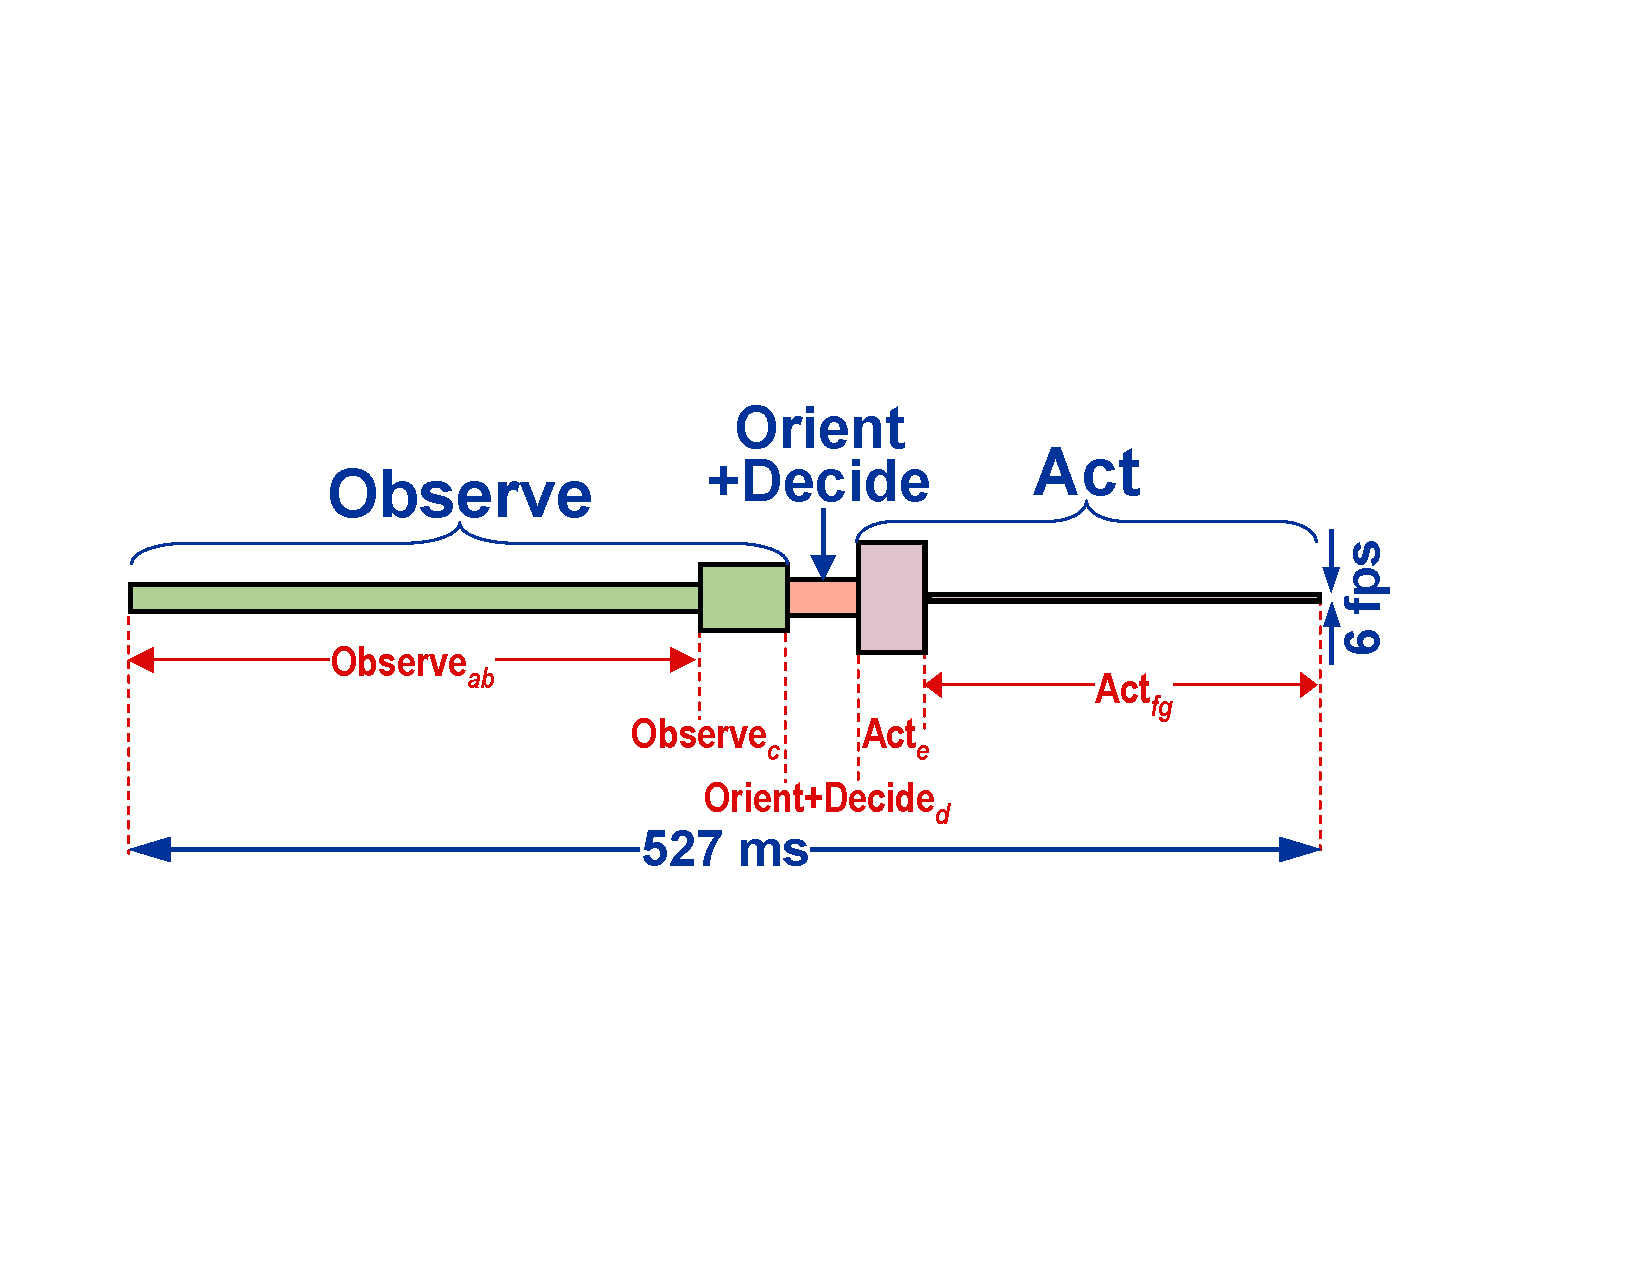
\includegraphics[width=1.0\linewidth]{FIGS/fig-ooda-scaling.pdf}
\begin{captext}
  This figure uses the same notation as Figure~\ref{fig:nomenclature},
  and color coding as Figure~\ref{fig:ooda-loop}.  Width is scaled to
  represent latency, and height to represent throughput.
  Orient+Decide$_d$ here assumes negligible application-specific
  processing.  For the electromechanical actuation represented by
  component Act$_{fg}$, the reciprocal of its latency is used as its
  throughput.
\end{captext}
\vspace{-0.1in}
\caption{\small \ooda~ Loop Latency \& Throughput}
\label{fig:ooda-scaling}
\vspace{-0.1in}
\end{figure}

\subsection{The Full \ooda~Loop}
\label{sec:e2e-discussion}

Using the same notation as Figure~\ref{fig:nomenclature}, a visual
summary of the measurements reported in \S\ref{sec:d2c-drone} to
\S\ref{sec:c2d-drone} is shown in Figure~\ref{fig:ooda-scaling}.  This
captures the best-case \ooda~loop, where no time is spent in Stage-2
and Stage-3 of Orient+Decide$_d$.  In practice, it is those stages that
perform the processing for drone autonomy such as object detection,
object tracking, Kalman filtering, and route planning.  They also do
the processing to generate the commands for drone actuation such as
gimbal movement, flight path alteration, or altitude change.  The
height and width of the resulting Orient+Decide$_d$ component in
Figure~\ref{fig:ooda-scaling} would need to be scaled to include such
application-specific processing.  In some cases, that component
may dominate the entire \ooda~loop.

In a typical application, many iterations of the \ooda~loop may
involve no actuation, thus eliminating Act$_{e}$ and Act$_{fg}$.  For
example, consider a target that is moving in a straight line at
constant speed.  Successive \ooda~loops of a drone that is following
that target only need to confirm that it remains centered in the FOV.
Only abrupt change of motion by the target will stress the \ooda~loop.
Fast reaction is then needed to discover that the target is
off-center, and to actuate the gimbal or drone to re-center it before
it is lost from the FOV.  Figure~\ref{fig:ooda-scaling} shows that the
latency and throughput of Observe$_{ab}$ are the limiting constraint
in uneventful settings.  It is thus the inherent attributes
of the drone, rather than network bandwidth or the cloudlet processing
power, that limits us today.

\begin{comment}
\begin{figure}
\centering
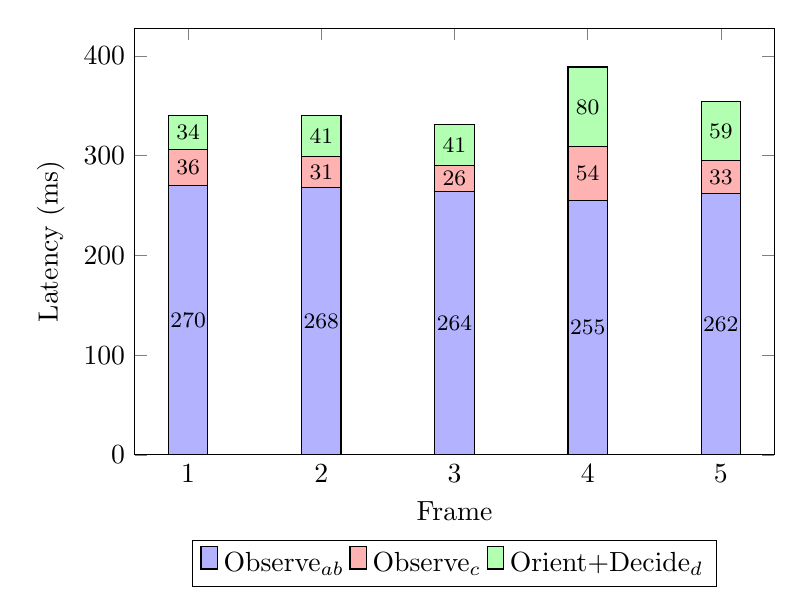
\begin{tikzpicture}
    \begin{axis}[
        ybar stacked,
        bar width=0.5cm,
        width=0.8\linewidth,
        height=7cm,
        ylabel={Latency (ms)},
        xlabel={Frame},
        symbolic x coords={1, 2, 3, 4, 5},
        xtick=data,
        ymin=0,
        legend style={at={(0.5,-0.2)},
                      anchor=north,legend columns=3},
        nodes near coords,
        every node near coord/.append style={font=\footnotesize, /pgf/number format/.cd, fixed, precision=1},
    ]
        \addplot+[ybar, color=black, fill=blue!30] plot coordinates {(1, 270) (2, 268) (3, 264) (4, 255) (5, 262)}; % Oberve_ab
        \addplot+[ybar, color=black, fill=red!30] plot coordinates {(1, 36) (2, 31) (3, 26) (4, 54) (5, 33)}; % Observe_c
        \addplot+[ybar, color=black, fill=green!30] plot coordinates {(1, 34) (2, 41) (3, 41) (4, 80) (5, 59)}; % Orient+Decide_d

        \legend{Observe$_{ab}$, Observe$_c$, Orient+Decide$_d$}
    \end{axis}
\end{tikzpicture}
\vspace{-0.1in}
\caption{\small{Latency Breakup by {\sc OODA} phase}}
\label{fig:latency-breakup}
\end{figure}

% If we show this stacked bar chart in terms of averages instead of the
% breakup for five example frames we can include the Act phase as well.
%
% So then there would be just one bar in the stacked bar chart.
\end{comment}


